% unicodeは、hyperrefへの指定で、pdfのメタデータにあるタイトルの文字化けを防ぐ
% ptは細かい指定はできないらしい
% チートシート
% https://www.cpt.univ-mrs.fr/~masson/latex/Beamer-appearance-cheat-sheet.pdf
\documentclass[unicode, 14pt, aspectratio=169]{beamer} 
\usepackage{minted}
\usepackage{listings}
\usepackage{enumitem}
\usepackage{xcolor}
\usepackage{textcomp}
\usepackage[backend=biber, style=ieee]{biblatex}
\usetheme{rikako}
\date{\number\year 年\number\month 月\number\day 日}
\addbibresource{main.bib}
\title{runcのUNIXプログラミング}
\author{\texttt{ryotaro612}}
\begin{document}
\usemintedstyle{titech}
\begin{frame}[noframenumbering, plain]
\titlepage
\end{frame}
\section{導入}
\begin{frame}
  \frametitle{runc}
  後にDockerから独立した低レベルなコンテナランタイムのCLI
  \begin{figure}
    \centering
    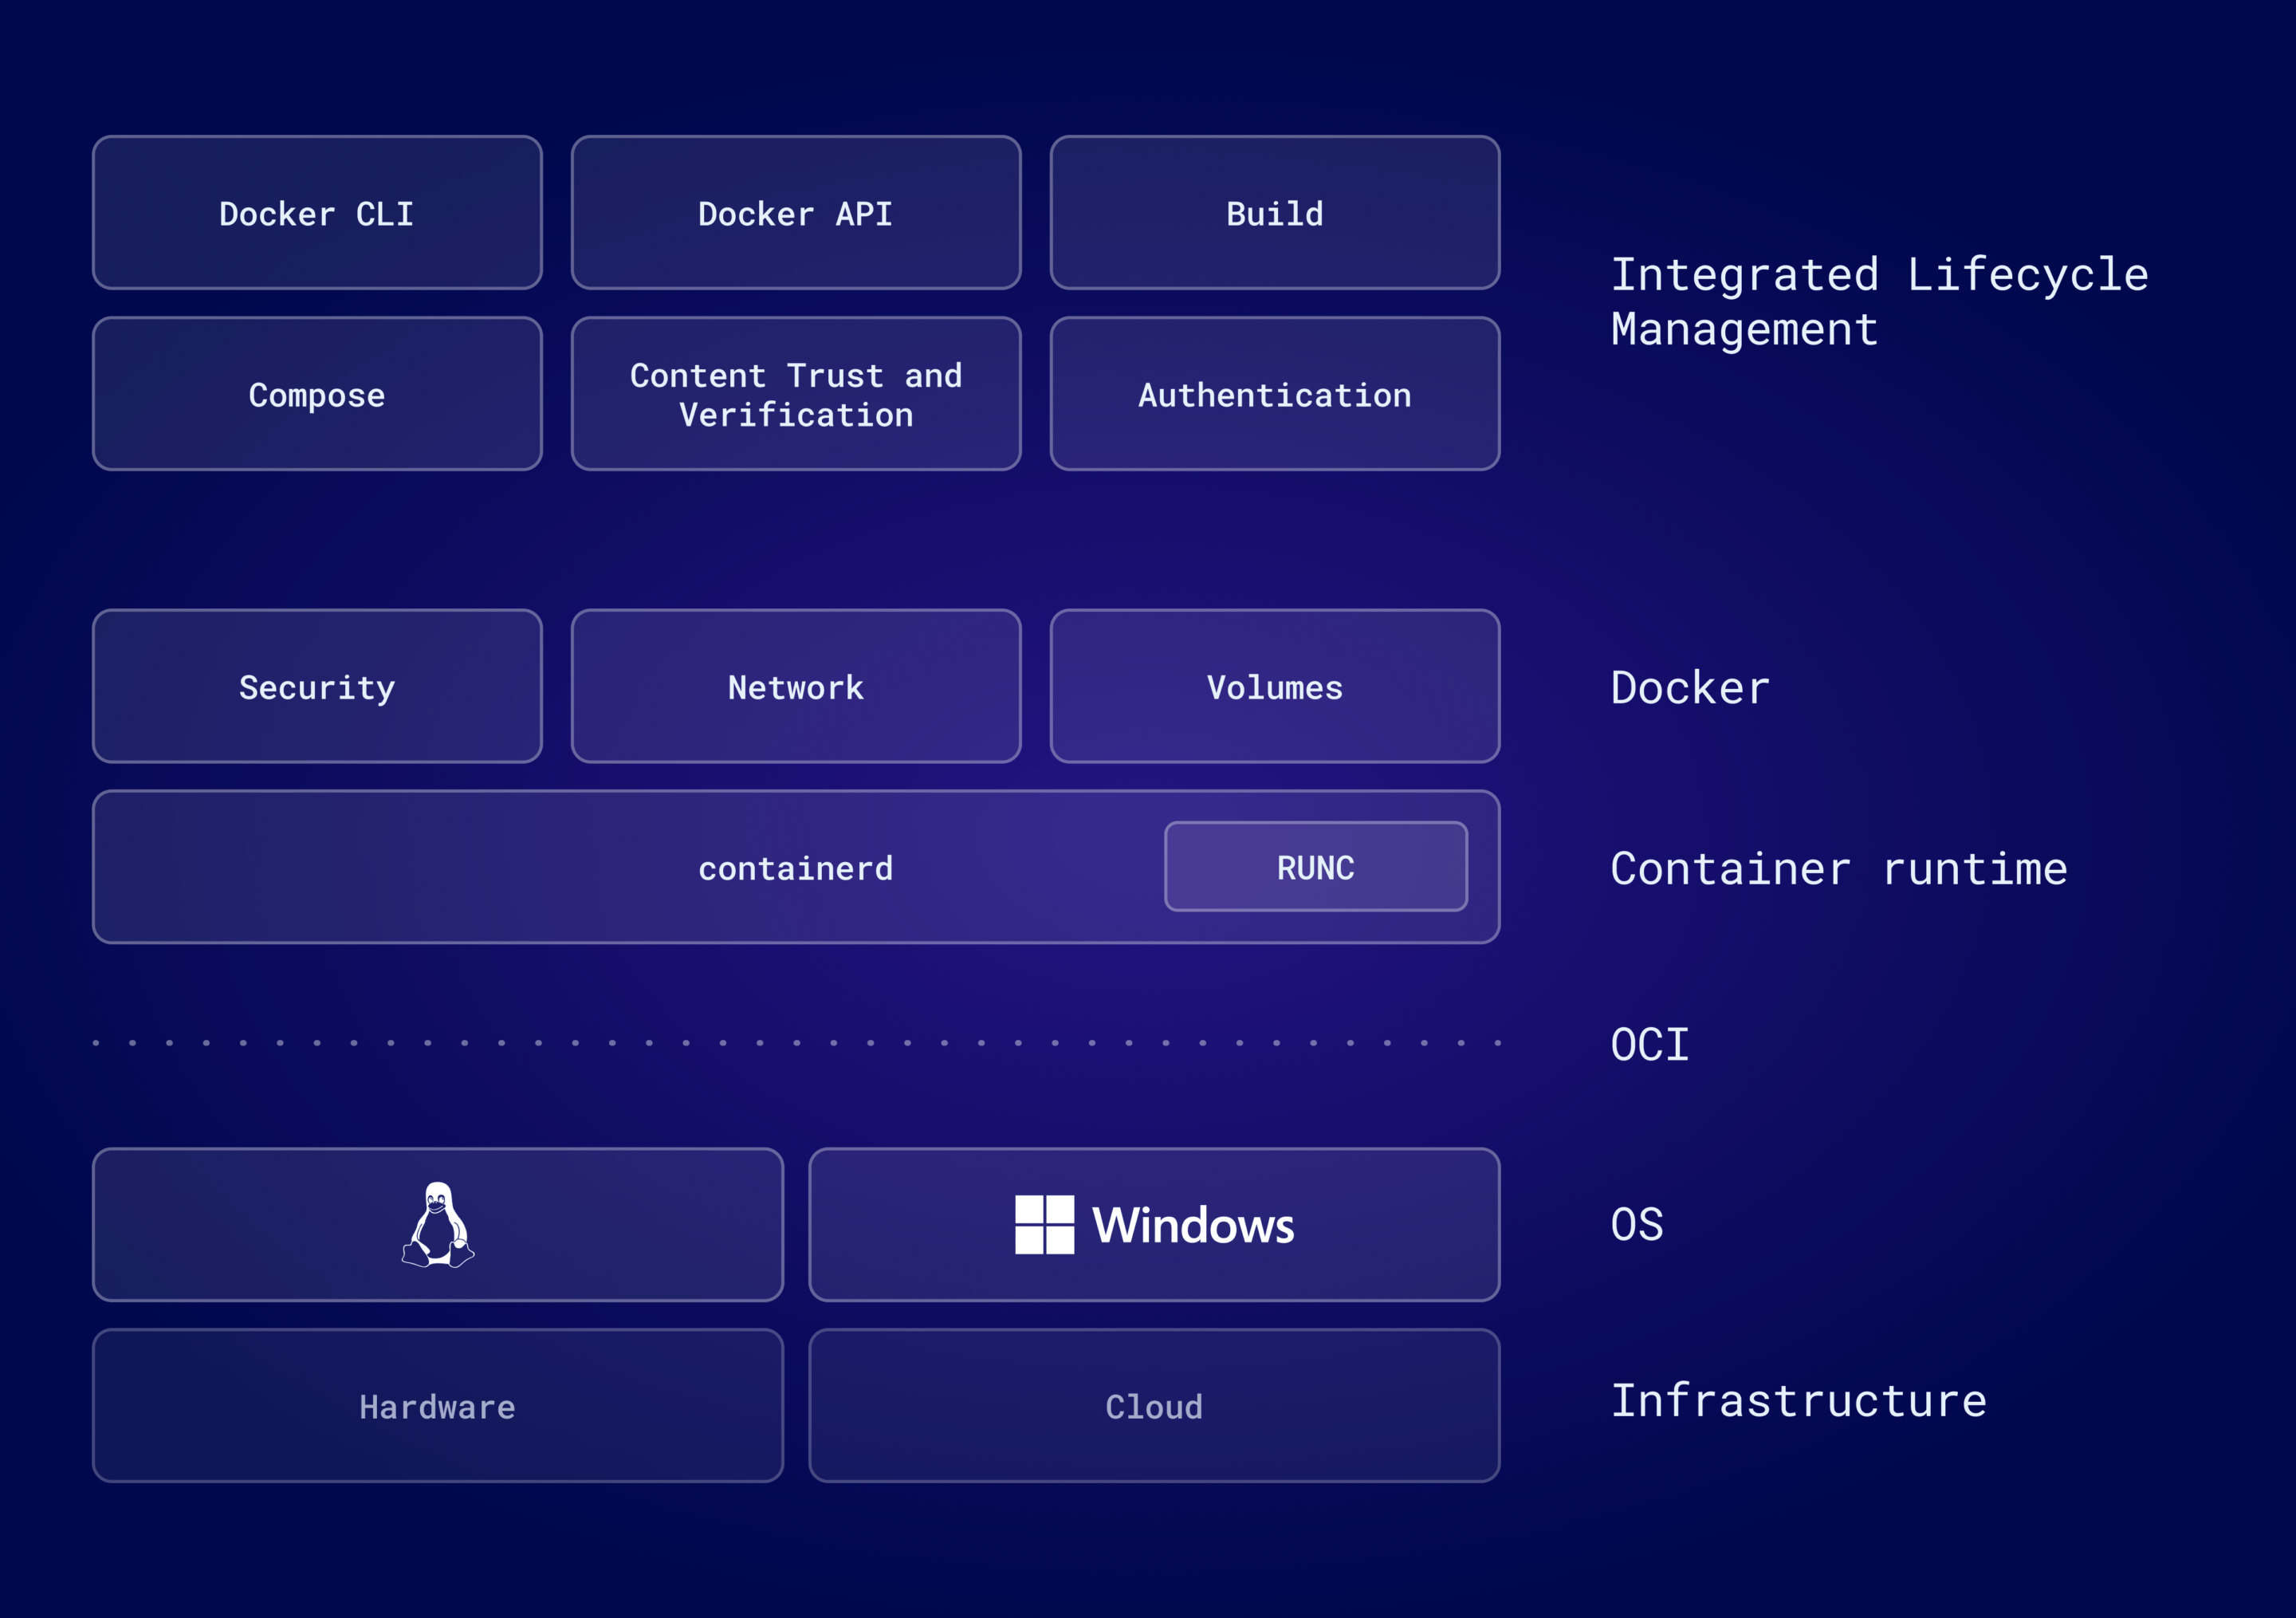
\includegraphics[width=6.8cm]{images/containerd-diagram-v1.png}
    \caption{Docker, runc, OSの階層\footnote{\scriptsize{\href{https://www.docker.com/blog/containerd-vs-docker}{containerd vs. Docker: Understanding Their Relationship and How They Work Together}より}}}
    \label{fig:runc}
  \end{figure}
\end{frame}
\begin{frame}%[fragile=singleslide]
  \frametitle{抽象度の低い\texttt{runc}}
  イメージはいらず、コンテナのルート\texttt{/}があればいい
  \begin{center}
    \inputminted[fontsize=\small]{sh}{code/run.sh}
    runcでコンテナの\texttt{sh}を開始\supercite{runc}  
  \end{center}
\end{frame}
\begin{frame}
  \frametitle{資料の目的}
  UNIXプログラミングの基本的な道具を知ること
  \begin{center}
    Infrastructure Plumbing Manifesto\footnote{\scriptsize{dockerのブログ \href{https://www.docker.com/blog/runc/}{Introducing runC: a lightweight universal container runtime
}より}}
    \end{center}
  \begin{quote}
    \begin{itemize}
    \item {\small When you need to create new plumbing, make it easy to re-use and contribute improvements back.}
    \item {\small Follow the unix principles: several simple components are better than a single, complicated one.}
    \item {\small Define standard interfaces which can be used to combine many simple components into a more sophisticated system.}
  \end{itemize}
\end{quote}
  runcはUNIXの原則による小さな機能を組み合わせ
\end{frame}
\begin{frame}
  \frametitle{runc runの手続き}
  runが実行したrunc initが\href{https://man7.org/linux/man-pages/man2/execve.2.html}{execve}でコンテナのプロセスになる
  \begin{figure}
    \centering
    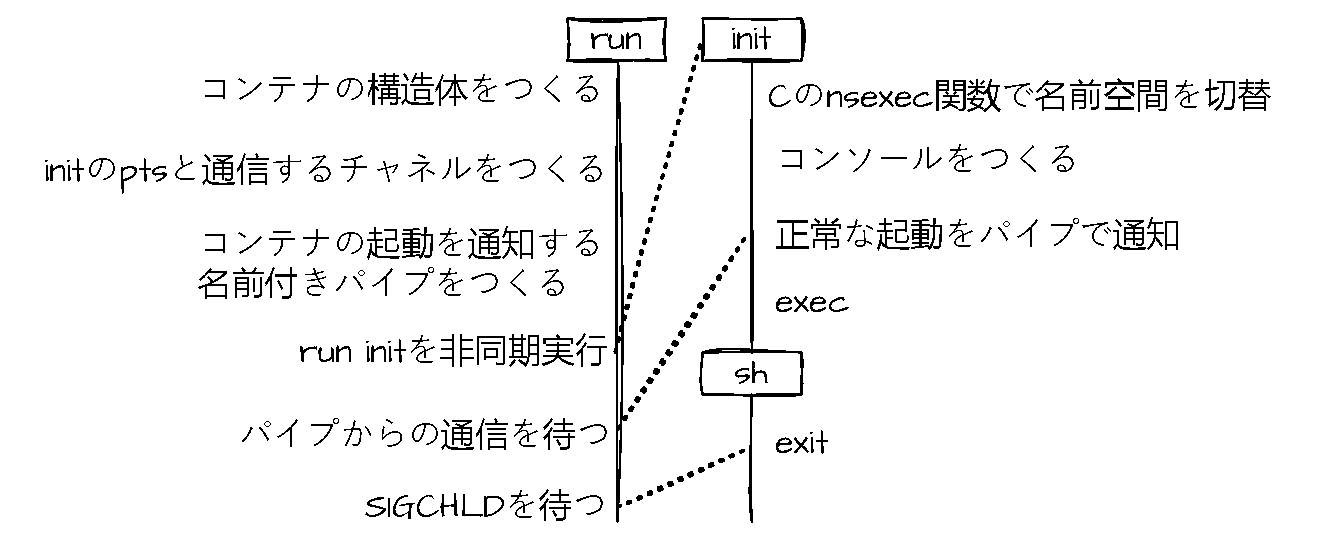
\includegraphics[width=13cm]{images/overview.drawio.pdf}
    \caption{runとinitコマンドの手続き\footnote{点線はプロセスを横断する処理}}
  \end{figure}
\end{frame}
\section{ホストとコンテナの端末間通信}
\begin{frame}[label=overview]
  \frametitle{再掲 runc runの手続き}
  \begin{figure}
    \centering
    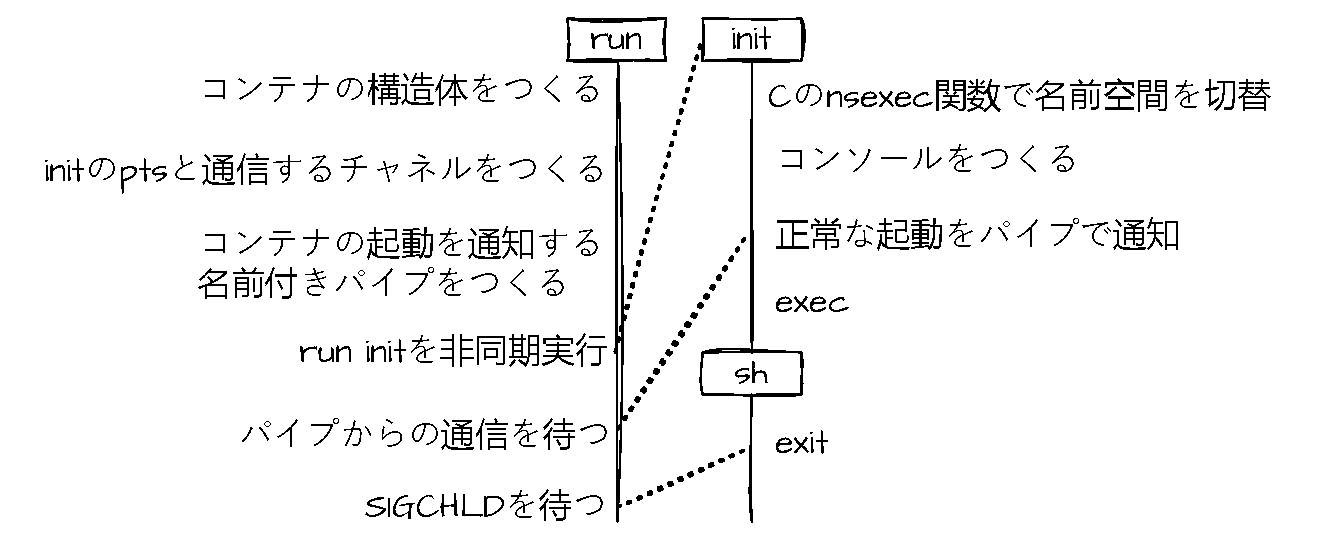
\includegraphics[width=14cm]{images/overview.drawio.pdf}
    \caption{runとinitコマンドの手続き\footnote{点線はプロセスを横断する処理}}
  \end{figure}
\end{frame}
\begin{frame}
  \frametitle{疑似端末 \texttt{pty}}
  \texttt{pty}はキャラクタデバイスのマスタ、スレーブの組\supercite{pty}
  \begin{itemize}[leftmargin=0.8cm,label=$\circ$]
  \item マスタ\texttt{/dev/ptmx}を開くと\texttt{/dev/pts}にスレーブができる
  \item 一方の入力が他方の出力になる
  \item \href{https://man7.org/linux/man-pages/man3/ptsname.3.html}{\texttt{ptsname}}関数にマスタのファイル記述子を渡すとスレーブをパスがわかる
  \item 通常、forkされたプロセスはスレーブを複製して標準I/O, エラー\footnote{\scriptsize{\texttt{ls -l /proc/<pid>/fd}で記述子0, 1, 2の参照先を確認できる}}にする\supercite{advancedunix}
  \end{itemize}
\end{frame}
\begin{frame}
  \frametitle{\texttt{pty}の準備}

  \texttt{runc init}は\texttt{runc run}にマスタのファイル記述子を送る
  \setlist[enumerate]{label*=\arabic*.,ref=\arabic*}
  \begin{enumerate}[leftmargin=1.2cm]
  \item \texttt{run}は\href{https://man7.org/linux/man-pages/man2/socketpair.2.html}{\texttt{socketpair}}でファイル記述子のペアをつくる。ペアは双方向通信できる
  \item \texttt{run}は\href{https://pkg.go.dev/os/exec\#Cmd}{\texttt{Cmd.ExtraFiles}}で記述子を1つ\texttt{init}にわたす 
  \item \texttt{init}は\texttt{/dev/ptmx}を開く
  \item \texttt{init}はsendmsgで記述子を介してマスタを\texttt{run}に送る
  \item \texttt{run}はマスタの入出力を標準IOにコピーする
  \end{enumerate}
\end{frame}
\begin{frame}
  \frametitle{\texttt{init}}
  マスタを\texttt{run}に送る
  \begin{center}
    \inputminted{go}{code/tty_init.go}
    \href{https://github.com/opencontainers/runc/blob/7cb363254b69e10320360b63fb73e0ffb5da7bf2/libcontainer/init_linux.go\#L371}{\texttt{setupConsole}}関数の抜粋
  \end{center}
\end{frame}
\begin{frame}
  \frametitle{\texttt{init}}
  \href{https://ja.manpages.org/dup3/2}{dup3}で標準IO, エラー出力のためにスレーブを複製
  \begin{center}
    \inputminted{go}{code/pty_init_dup.go}
    \href{https://github.com/opencontainers/runc/blob/7cb363254b69e10320360b63fb73e0ffb5da7bf2/libcontainer/console_linux.go\#L28}{\texttt{dupStdio}}関数の抜粋
  \end{center}
\end{frame}
\begin{frame}
  \frametitle{\texttt{init}}
  スレーブをプロセスの制御端末にする\supercite{ioctl}
  \begin{center}
    \inputminted{go}{code/pty_tty.go}
    \href{https://github.com/opencontainers/runc/blob/7cb363254b69e10320360b63fb73e0ffb5da7bf2/libcontainer/system/linux.go\#L121}{\texttt{Setctty}}関数の抜粋
  \end{center}
\end{frame}
\begin{frame}
  \frametitle{\texttt{run}}
  ホストの標準入力をマスタに書き、マスタの出力をホストの標準出力に送る
  \begin{center}
    \inputminted{go}{code/tty_run.go}
    \href{https://github.com/opencontainers/runc/blob/7cb363254b69e10320360b63fb73e0ffb5da7bf2/tty.go\#L102}{\texttt{recvtty}}関数の抜粋
  \end{center}
  \href{https://man7.org/linux/man-pages/man7/epoll.7.html}{\texttt{epoll}}でマスタの入出力を監視
\end{frame}
\section{名前空間}
\begin{frame}
  \frametitle{名前空間\supercite{namespaces}}
  空間のプロセスには自分達がリソースを占有したように見える
  \begin{itemize}[leftmargin=0.8cm,label=$\circ$]
    \item マウントポイント、プロセスIDなど6種類の名前空間がある
    \item 名前空間の間でリソース名が重複しても互いに影響しない
    \item API
      \begin{description}[leftmargin=4.8em,style=nextline]
      \item[\texttt{clone}] 新しいプロセスを作る。子プロセスを新しい名前空間に入れることもできる
      \item[\texttt{setns}] 呼びだしたスレッドを既存の名前空間に入れる。用途はコンテナ間でのネットワークの共有など
      \item[\texttt{unshare}] 指定した種類の名前空間を作り、呼びだしたプロセスを移動する
      \end{description}
    \end{itemize}
\end{frame}
\begin{frame}
  \frametitle{\texttt{nsexec}で\texttt{init}の名前空間を移動}
  Goの前にCの\texttt{nsexec}関数を実行する
  \begin{center}
    \inputminted{go}{code/nsenter.go}
    \href{https://github.com/opencontainers/runc/blob/7cb363254b69e10320360b63fb73e0ffb5da7bf2/libcontainer/nsenter/nsenter.go\#L12}{\texttt{nsenter.go}}の抜粋
  \end{center}
  \texttt{setns}はスレッドの名前空間を移すが、Goのランタイムには複数のスレッドがある
\end{frame}
\begin{frame}
  \frametitle{\texttt{nsexec}}
  \texttt{clone}をして名前空間を移動する
  \begin{columns}
    \begin{column}{0.5\textwidth}
      \begin{itemize}[leftmargin=0.8cm,label=$\circ$]
      \item \href{https://man7.org/linux/man-pages/man2/clone.2.html}{\texttt{clone}}に\texttt{CLONE\_PARENT}を渡すので、新しい\texttt{init}の親プロセスは、呼出元\texttt{init}の親プロセス\texttt{run}になる。結果、\texttt{SIGCHLD}が\texttt{run}に送られる
      \item \texttt{uid\_map}, \texttt{gid\_map}には、
      \end{itemize}
    \end{column}
    \begin{column}{0.5\textwidth}
      \begin{figure}
        \centering
        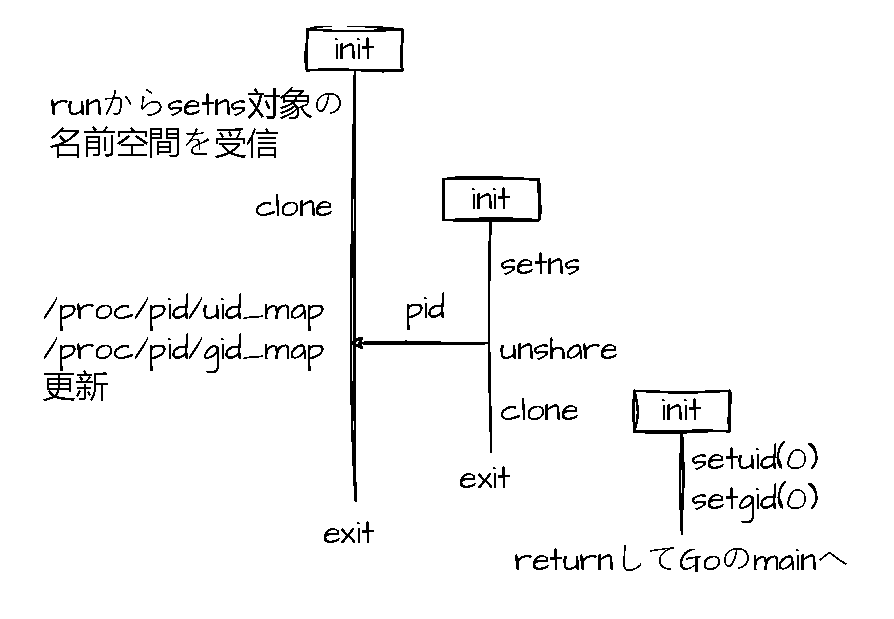
\includegraphics[width=7cm]{images/nsenter.drawio.pdf}
        \caption{\texttt{nsexec}の処理手順}
        \label{fig:nsenter}
      \end{figure}      
    \end{column}
  \end{columns}
\end{frame}
\section{ファイルシステムの変更}
\begin{frame}[t]
  \frametitle{\texttt{init}のルートファイルシステムを変更}
  \texttt{pivot\_root}でファイルシステムを変更する
  \begin{center}
    \inputminted{sh}{code/pivot_root.sh}
    \texttt{pivot\_root}の実行例
  \end{center}
\end{frame}
\section{付録 コンテナの構造体}
\begin{frame}
  \frametitle{libcontainer.Container}
  フィールドは非公開
  \begin{columns}
    \begin{column}{0.5\textwidth}
      \begin{center}
        \inputminted{go}{code/container.go}
        libcontainer.Container\supercite{libcontainer}
      \end{center}
    \end{column}
    \begin{column}{0.5\textwidth}  %%<--- here
      \begin{itemize}[leftmargin=0.2cm,label=$\circ$]
        \item \texttt{stateDir}は\texttt{runc}の\texttt{--root}オプション\texttt{<dir>}とすると\texttt{<dir>/<id>}
        \item \texttt{stateDir}には\texttt{run init}を呼びだす \texttt{/proc/self/exe}の複製や名前つきパイプをおく
        \item \texttt{/proc/self/exe}は実行中のプログラムのパスのシンボリックリンク
      \end{itemize}
    \end{column}
  \end{columns}
\end{frame}
\begin{frame}
  プロセスの非機能を隔離、監視\supercite{rdt}する
  \frametitle{libcontainer.Container}
  \begin{center}
    \inputminted{go}{code/container2.go}
    libcontainer.Container\supercite{libcontainer}
  \end{center}
\end{frame}
\begin{frame}
  コンテナで実行したいプロセスの情報がある
  \frametitle{libcontainer.Container}
  \begin{center}
    \inputminted{go}{code/container3.go}
    libcontainer.Container\supercite{libcontainer}
  \end{center}
\end{frame}
\begin{frame}[t]
  \frametitle{libcontainer.Container}
  コンテナのチェックポイント、リストアのフィールドがある\supercite{criu}
  \begin{center}
    \inputminted{go}{code/container4.go}
    libcontainer.Container\supercite{libcontainer}
  \end{center}
\end{frame}
\begin{frame}[allowframebreaks]
  \frametitle{参考資料}
  \printbibliography
  % 引用していないbibファイルの要素も記載する  
  \nocite{*} 
\end{frame}
\end{document}
